\section{Introduction - Networking Technologies}

\begin{frame}{OSI Model}
	\begin{columns}
	\column{0.2\textwidth}
		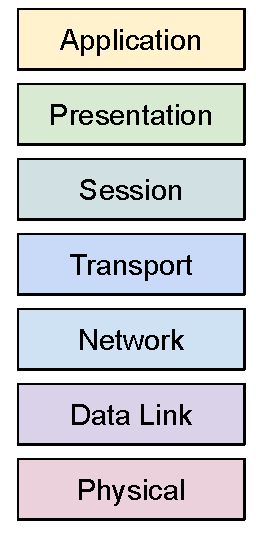
\includegraphics[width=0.9\textwidth]{slides/networking-stack-overview/osi.pdf}
	\column{0.8\textwidth}
	\begin{itemize}
		\item \textbf{O}pen \textbf{S}ystems \textbf{I}nterconnection
		\item Reference model to design network protocols, created in the late 1970s
		\item Defines 7 \textbf{layers}, with specific functions and semantics
		\item Each layer relies on the layer below, and provides features to the layer above
			\begin{itemize}
				\item In practise, this is done through \textbf{encapsulation}
				\item Each layer add its required data at the front of the data array
					\begin{itemize}
						\item This is the layer's \textbf{header}
					\end{itemize}
				\item A Layer N's header is part of Layer N-1's payload
			\end{itemize}
	\end{itemize}
	\end{columns}
\end{frame}

\begin{frame}{OSI layer communication}
	\begin{columns}
	\column{0.2\textwidth}
		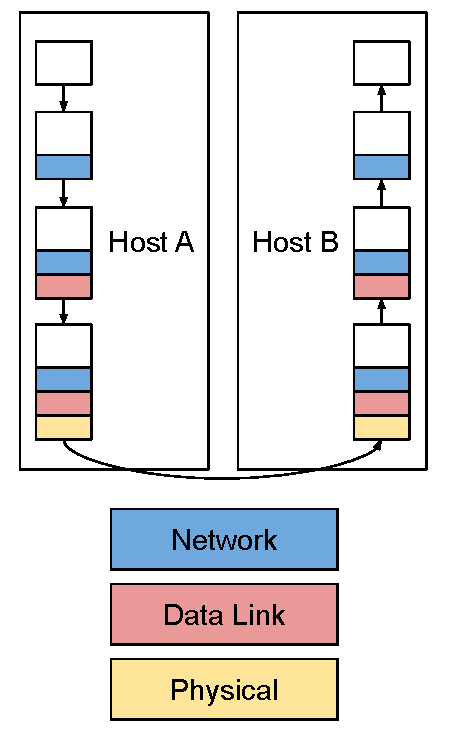
\includegraphics[width=1.2\textwidth]{slides/networking-stack-overview/osi_encap.pdf}
	\column{0.8\textwidth}
	\begin{itemize}
		\item The payload sent by a layer targets the same layer on the receiving end
		\item Each layer only cares about its specific header and treats the payload as a \textbf{black box}
		\item When the \textbf{peer} receives it, it \textbf{decapsulates} the received data
		\item Every layer has its own semantics about the data it manipulates
		\item Every layer's unit is called \textbf{P}rotocol \textbf{D}ata \textbf{U}nit
		\item Every layer has a \textbf{M}aximum \textbf{T}ransmit \textbf{U}nit per PDU
	\end{itemize}
	\end{columns}
\end{frame}

\begin{frame}{Layer 1 - PHY Layer}
	\begin{itemize}
		\item Defines how data is sent to a peer trough a \textbf{physical medium}
		\item PDU is \textbf{symbols} and \textbf{bits}
		\item IEEE 802.3 "Ethernet" defines a lot of Layer 1 technologies
			\begin{itemize}
				\item 1000BaseT4 : Transmit data at 1000Mbps over 4 twisted copper pairs
				\item 1000BaseFX : Transmit data at 1.25Gsps / 1Gbps over an optics fiber
				\item 10BaseT1S : Transmit data at 10Mbps over a single twisted copper pair
				\item Ethernet protocols may use the same medium
					\begin{itemize}
						\item Protocol selection can be done through \textbf{autonegotiation}
						\item Link detection is done by sending \textbf{Idle} words
					\end{itemize}
			\end{itemize}
		\item IEEE 802.11 "Wifi" also defines Layer 1 technologies using 2.4/5/60GHz radio modulation
		\item Many more exists : IEEE 802.15.4, "Bluetooth", NFC, etc.
		\item Usually handled by a dedicated hardware component : a \textbf{PHY}
	\end{itemize}
\end{frame}

\begin{frame}{Layer 2 - Data Link Layer}
	\begin{itemize}
		\item Sometimes called \textbf{MAC} layer
		\item PDU is a \textbf{Frame}
		\item In charge of Point-to-point communication
		\item IEEE 802.3 "Ethernet" defines a Layer 2 standard as well
			\begin{itemize}
				\item Source address, Destination address, Layer 3 type
			\end{itemize}
		\item IEEE 802.11 "Wifi" also defines a Layer 2
			\begin{itemize}
				\item 2, 3 or 4 addresses
				\item Receiver, Transmitter, Source and Destination
			\end{itemize}

	\end{itemize}
\end{frame}

\begin{frame}{Ethernet - Layer 2}
	\begin{center}
	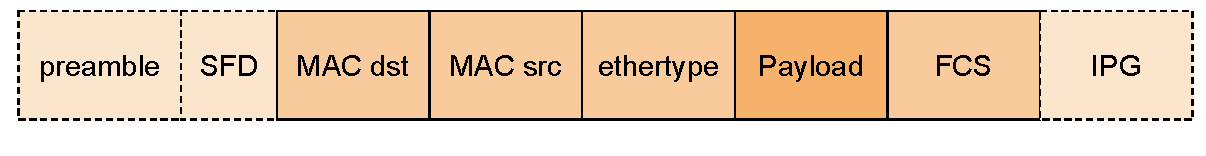
\includegraphics[width=0.7\textwidth]{slides/networking-stack-overview/ethernet_frame.pdf}
	\end{center}
	\begin{itemize}
		\item Point-to-point \textbf{frames} are sent on the medium, separated by a \textbf{gap}
		\item Regardless of the speed and medium, frames have the same structure :
			\begin{itemize}
				\item 7 bytes \textbf{Preamble}: Used to synchronize both equipments
				\item 1 byte \textbf{SFD} (Start Frame Delimiter): Ends the preamble
				\item 6 bytes \textbf{Destination address}, identifying the destination equipment
				\item 6 bytes \textbf{Source address}, identifying the source equipment
				\item 2 bytes \textbf{ethertype}, identifying the encapsulated protocol
				\item A \textbf{payload}
				\item 4 trailing bytes \textbf{FCS} (Frame Check Sequence): Checksum of the frame
			\end{itemize}
		\item Each frame must be separated by at least 12 bytes, named the \textbf{I}nter \textbf{P}acket \textbf{G}ap
		\item $header + payload + fcs <= 1522$ bytes, the payload's size is at most \textbf{1504 bytes}
		\item $header + payload + fcs >= 64$ bytes, the payload must be \textit{zero-padded} otherwise
	\end{itemize}
\end{frame}

\begin{frame}{Network Bridging}
	\begin{itemize}
		\item A \textbf{Network bridge} is a Layer 2 device interconnecting multiple network segments
		\item We usually use a dedicated \textbf{Network Switch} for this purpose
			\begin{itemize}
				\item Using a \textbf{ASIC} chip
				\item Using a software implementation
			\end{itemize}
		\item Ethernet switches are usually \textbf{transparent switches}
			\begin{itemize}
				\item They monitor Layer 2 header to \textbf{learn} the Port to Address assciation
				\item This is stored in the FDB : \textbf{F}orwarding \textbf{D}ata\textbf{B}ase
			\end{itemize}
		\item Some switches can be highly configurable, and support \text{VLAN}s
	\end{itemize}
	% Bridge, switch, 
\end{frame}

\begin{frame}{Transparent bridge}
	\begin{columns}
		\column{0.3\textwidth}
		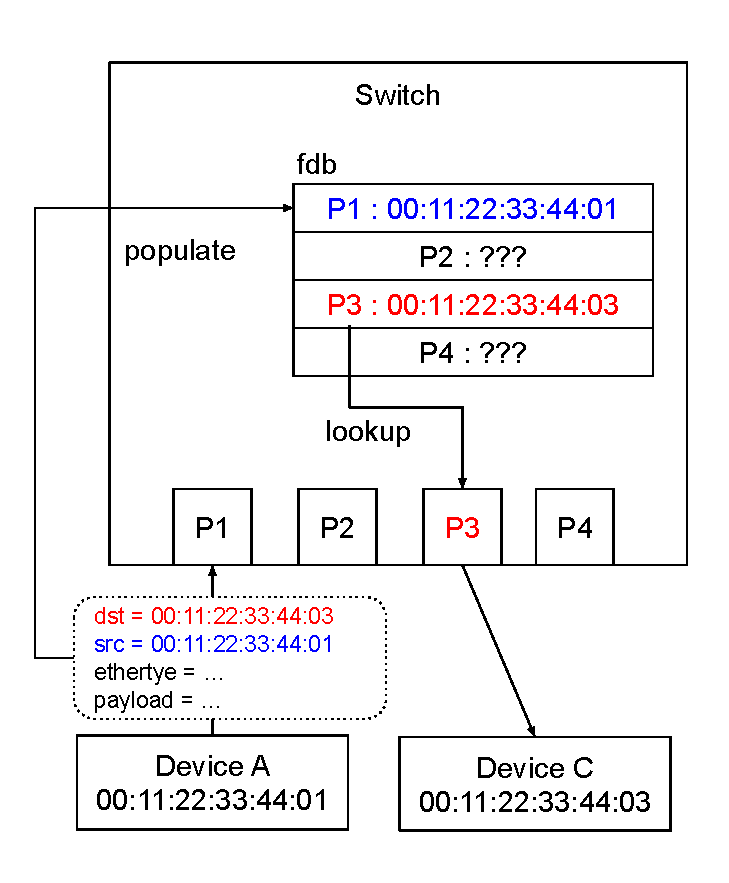
\includegraphics[width=1.1\textwidth]{slides/networking-stack-overview/transparent_bridge.pdf}
		\column{0.7\textwidth}
		\begin{itemize}
			\item Ports are monitored, the \textbf{source address} saved
			\item The \textbf{destination address} is looked-up
			\item If no match is found, the frame is \textbf{flooded} on all ports
			\item Advanced switches can do \textbf{port mirroring}
				\begin{itemize}
					\item Duplicate traffic going forwarded a port to another port
					\item Used for administration and troubleshooting
				\end{itemize}
		\end{itemize}
	\end{columns}
\end{frame}

\begin{frame}{VLANs}
	\begin{columns}
		\column{0.3\textwidth}
			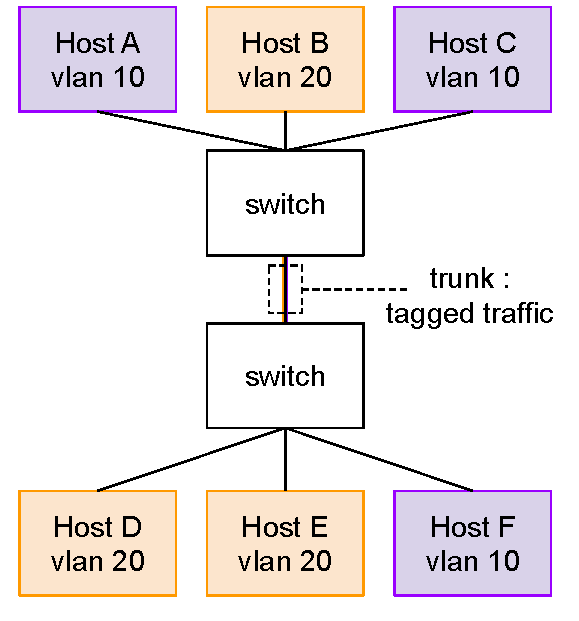
\includegraphics[width=1.1\textwidth]{slides/networking-stack-overview/vlan_topo.pdf}
		\column{0.7\textwidth}
	\begin{itemize}
		\item \textbf{V}irtual \textbf{L}ocal \textbf{A}rea \textbf{N}etwork
		\item Multiple VLAN technologies exist:
			\begin{itemize}
				\item 802.1Q (\textit{dot1q}): Layer 2
				\item 802.1AD (\textit{QinQ}): Layer 2
				\item VxLan : Layer 4 (UDP)
				\item MACVlan : Based only on MAC addresses
			\end{itemize}
		\item Logical segmentation of the network
		\item Used for isolation, priorisation and bandwitdh optimisation
		\item The same conduit can be used to convey multiple VLANs
			\begin{itemize}
				\item We talk about a \textbf{trunk} interface
				\item Frames are \textbf{tagged} to indicate the VLAN it belongs to
			\end{itemize}
	\end{itemize}
	\end{columns}
\end{frame}

\begin{frame}{VLAN - 802.1Q}
	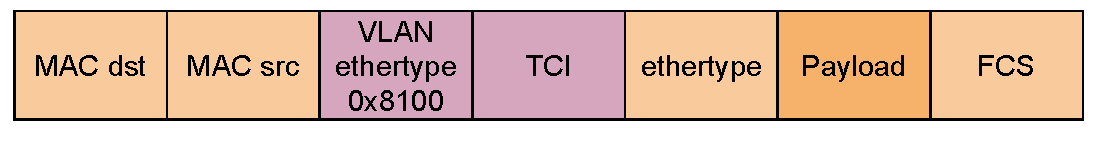
\includegraphics[width=0.8\textwidth]{slides/networking-stack-overview/ethernet_frame_vlan.pdf}

	\begin{itemize}
		\item A 802.1Q frame has includes an extra \textbf{4 bytes} tag in the Ethernet header
		\item The \textbf{ethertype} is set to \code{0x8100}, the real ethertype is stored after the tag
		\item A 16 bits value identifies the Tag : \textbf{T}ag \textbf{C}ontrol \textbf{I}nformation
			\begin{itemize}
				\item 3 bits indicate a \textbf{priority}, between 0 and 7
					\begin{itemize}
						\item Also called \textbf{C}lass \textbf{o}f \textbf{S}ervice
					\end{itemize}
				\item 1 bit \textbf{D}rop \textbf{E}ligible \textbf{I}ndicator
				\item 12 bits represent the ID of the vlan, between 1 and 4094
					\begin{itemize}
						\item ID 0 means \textbf{no tag}, only the priorty is consided
						\item ID \textbf{4095} is reserved.
					\end{itemize}
			\end{itemize}
	\end{itemize}
	% Tag,QinQ, trunk, switch
\end{frame}

\begin{frame}{Layer 3 - Network Layer}
	\begin{itemize}
		\item PDU is \textbf{packet} or \textbf{Segment}
		\item Handles routing between multiple machines
		\item Defined by \textbf{subnets}, linked tothegher by \textbf{routers}
		\item Main technologies are \textbf{IPv4} and \textbf{IPv6}
			\begin{itemize}
				\item IPv4 : 32-bits addresses, IPv6 : 128-bits addresses
			\end{itemize}
		\item Layer 2 to Layer 3 addresses can be associated
			\begin{itemize}
				\item e.g. the \textbf{A}ddress \textbf{R}esolution \textbf{P}rotocol
				\item MAC to IP tables are named \textbf{ARP} or \textbf{neighbouring} tables
			\end{itemize}
		\item Layer 3 can perform \textbf{fragmentation}
			\begin{itemize}
				\item e.g. if an IPv4 packet is too big to fit within the Ethernet MTU, it is split into multiple IPv4 packets
				\item each packet is individually routable
				\item Re-assembly is done by the peer
			\end{itemize}
	\end{itemize}
	%IPv4 IPv6 routing frag
\end{frame}

\begin{frame}{Transport Layer}
	\begin{itemize}
		\item Communication between endpoints over a routed network
			\begin{itemize}
				\item \textit{e.g.} Multple applications on the same machine
				\item Each end-point is further identified within the host 
				\item on TCP and UDP, \textbf{ports} are used
			\end{itemize}
		\item TCP : Connection-oriented, reliable, guarantees ordering.
			\begin{itemize}
				\item Stream of data, boundaries may be be preserved 
			\end{itemize}
		\item UDP : Connection-less, not reliable, no ordering guarantee
			\begin{itemize}
				\item Sends datagrams with clear boundaries
			\end{itemize}
		\item QUIC : Based on UDP, introduced by Google. Connection-oriended, reliable, guarantees ordering
			\begin{itemize}
				\item Can batch Acknowledgments, supports encryption (i think)
			\end{itemize}

	\end{itemize}
	%TCP UDP Srange stuff like QUIC
\end{frame}

\begin{frame}{Tunneling}
	\begin{columns}
	\column{0.3\textwidth}
		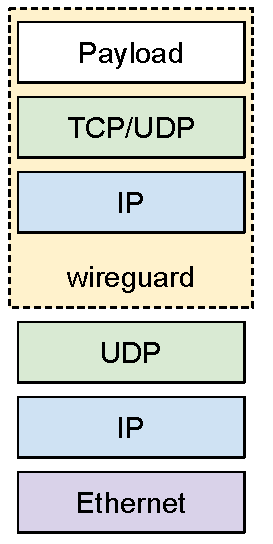
\includegraphics[width=0.8\textwidth]{slides/networking-stack-overview/wireguard.pdf}
	\column{0.7\textwidth}
	\begin{itemize}
		\item Encapsulate a Lower-level layer into a higher one
		\item Used to virtualise networks (e.g. VXLAN is Ethernet over UDP)
		\item Also used for encryption (IPSec, Wireguard, OpenVPN)
			\begin{itemize}
				\item \textit{e.g.} Wireguard Encrypts and encapsulates IP packets into UDP packets
			\end{itemize}
		\item There may therefore be more headers to decapsulate than there are ISO layers
	\end{itemize}
	\end{columns}
\end{frame}

\begin{frame}{Layers 5, 6 and 7}
	\begin{itemize}
		\item Session : Handles the connection, authentication and lifetime of data exchanges
			\begin{itemize}
				\item \textit{e.g.} RPC, SOCKS
			\end{itemize}
		\item Presentation : Handles the data conversion and serialization for interoperability
			\begin{itemize}
				\item \textit{e.g.} character transcoding depending on the locale
				\item \textit{e.g.} serializing user data in \code{JSON} or \code{XML}
			\end{itemize}
		\item Application : Communication between user applications
			\begin{itemize}
				\item \textit{e.g.} HTTP for Web applications
			\end{itemize}
		\item \textit{less relevant for this training, as they aren't handled by the linux kernel}
	\end{itemize}
\end{frame}

\section{The Linux Kernel Networking Stack}

\begin{frame}{The Linux Kernel Networking Stack}
	\begin{columns}
		\column{0.7\textwidth}
		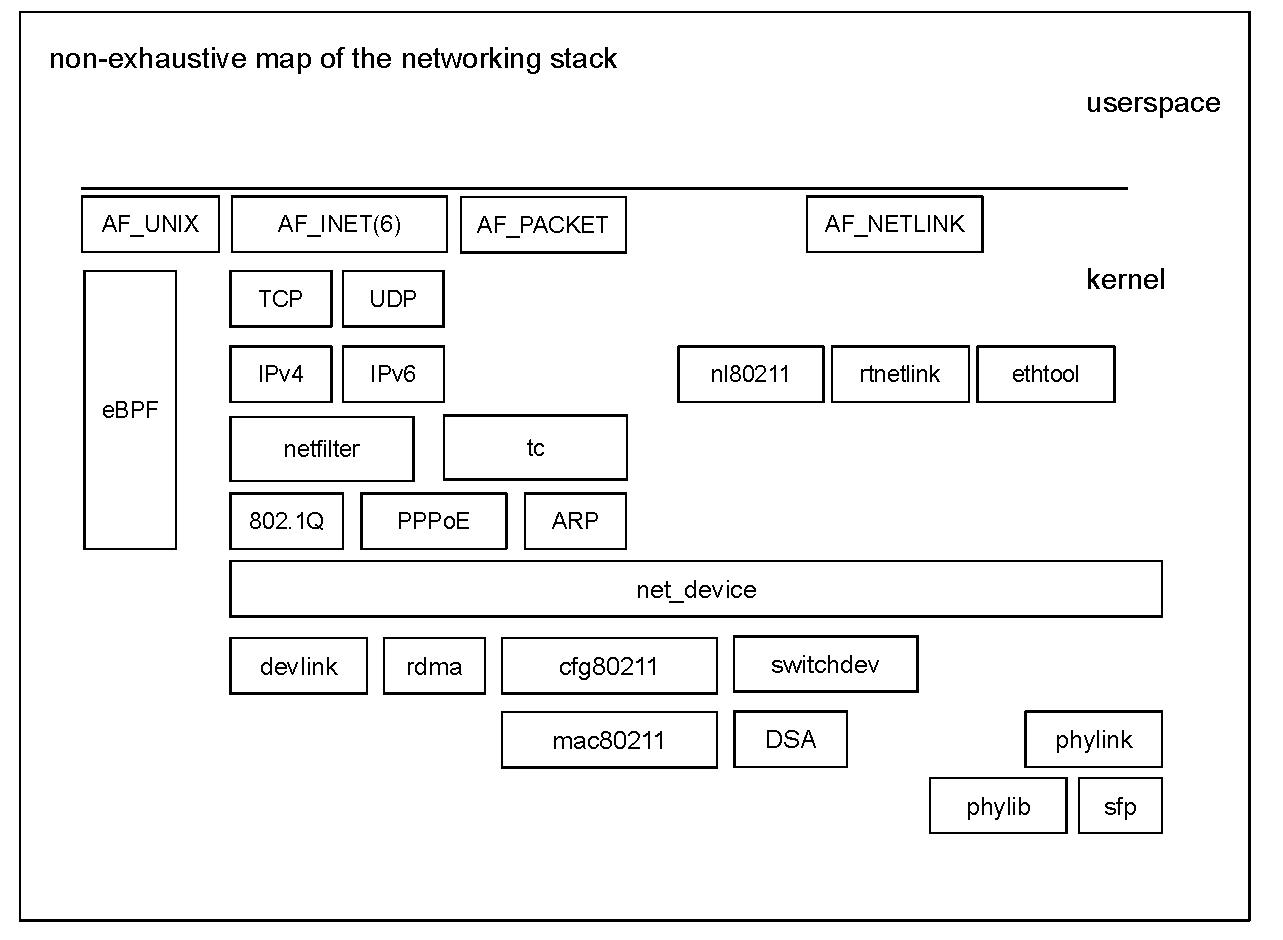
\includegraphics[width=\textwidth]{slides/networking-stack-overview/stackmap.pdf}
		\column{0.3\textwidth}
		As of v6.16-rc1 :
		\begin{itemize}
			\item over 209000 commits
			\item over 7750 files
			\item over 993000 LoC
			\item around 100 maintainers
			\item Around 880 drivers (Layer 2)
		\end{itemize}
	\end{columns}
\end{frame}

\begin{frame}{Some history}
	\begin{itemize}
		\item First support was introduced in v0.96 (may 1992) !
		\item Already exposing a socked-based API
		\item IPv4 : v0.98 - September 1992
		\item TCP/UDP : v0.98 - September 1992
		\item IPv6 : v2.2 - January 1999 (IPv6 was created in 1998)
		\item BPF : v2.5 - 2003, was then known as \textbf{L}inux \textbf{S}ocket \textbf{F}iltering
			\begin{itemize}
				\item eBPF : v3.15 - June 2014
			\end{itemize}
		\item PHYlib : v2.6.13 - August 2005, before that PHYs were handled in MAC drivers
		\item XDP : v4.8 - September 2016
		\item phylink : v4.13 - September 2017
	\end{itemize}
\end{frame}

\begin{frame}{Networking in the Linux Kernel}
	\begin{columns}
	\column{0.4\textwidth}
	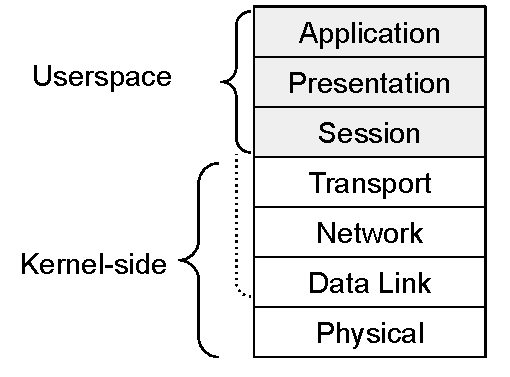
\includegraphics[width=\textwidth]{slides/networking-stack-overview/osi-kernel.pdf}
	\column{0.6\textwidth}
	\begin{itemize}
		\item Abstracts the Network Devices
		\item Implements some OSI Layers :
			\begin{itemize}
				\item Layer 1 (PHY) : Ethernet, WiFi, CAN, etc.
				\item Layer 2 (MAC) : Bridging, VLANs, etc.
				\item Layer 3 (Network) : IPv4, IPv6, etc.
				\item Layer 4 (Transport) : TCP, UDP, etc.
			\end{itemize}
		\item Provides a set of APIs to userspace :
			\begin{itemize}
				\item Socket API and \code{io_uring}
				\item Control through ioctl and Netlink
			\end{itemize}
	\end{itemize}
	\end{columns}
\end{frame}

\begin{frame}{Physical and MAC support}
	\begin{itemize}
		\item The Networking stack provides a framework for Layer 2 drivers : \kstruct{net_device}
		\item Used by Ethernet, Wifi, Bluetooth, CAN, 802.15.4, Radio, etc.
		\item PHY drivers have their dedicated frameworks
			\begin{itemize}
				\item phylib for Ethernet PHYs
				\item mac80211 and wiphy for 802.11 PHYs
			\end{itemize}
		\item A lot of communication technologies are handled through the network stack
			\begin{itemize}
				\item Ethernet
				\item Wifi
				\item Bluetooth and Bluetooth Low Energy
				\item Infiniband
				\item 802.15.4, radio, X.25
				\item CAN Bus
			\end{itemize}
	\end{itemize}
\end{frame}

\begin{frame}{Ethernet}
	\begin{itemize}
		\item Ethernet MAC controllers are supported through regular \kstruct{net_device} as well as \code{ethtool}
		\item Switch drivers are supported, with offload operation going through \href{https://docs.kernel.org/networking/switchdev.html}{Switchdev}
		\item Standalone Ethernet Switches are handled through \href{https://docs.kernel.org/networking/dsa/dsa.html}{DSA}
		\item Ethernet PHYs are supported via \href{https://docs.kernel.org/networking/phy.html}{phylib}, and the MAC to PHY link via \href{https://docs.kernel.org/networking/sfp-phylink.html}{phylink}
		\item SFF and SFP cages and modules are also supported
		\item Supports 802.3 frames and Ethernet II
		\item Multiple 802.1 and 802.3 Low-Level aspects are supported :
			\begin{itemize}
				\item Vlan with 802.1Q and 802.1AD
				\item Bridging and Switching
				\item MACSec (802.1ae) for Ethernet-level encryption
				\item Teaming, Bonding, HSR and PRP for link redudancy
			\end{itemize}
		\item Raw Ethernet frames can be sent and received in userspace API with \code{AF_PACKET}
	\end{itemize}
\end{frame}

\begin{frame}{Wireless subsystem}
	\begin{itemize}
		\item Wifi (802.11) Stack :
			\begin{itemize}
				\item Supports Wifi chips with internal MAC stack (\textbf{hardmac})
				\item Also provides a 802.11 MAC stack for \textbf{softmac} drivers in \code{mac80211}
				\item The main implementation is in \code{cfg80211}, configured via \code{nl80211}
			\end{itemize}
		\item Bluetooth stack :
			\begin{itemize}
				\item Low-level support for Bluetooth and BLE
				\item Exposes a socket-based API for management and data
				\item Profiles are implemented either in the kernel or userspace
				\item BlueZ is the main userspace companion stack
			\end{itemize}
		\item 802.15.4 stack :
			\begin{itemize}
				\item Also provides \textbf{hardmac} and \textbf{softmac} support
				\item Has its own PHY layer
				\item Complemented by the \textbf{6lowpan} stack for upper levels
					\begin{itemize}
						\item 6lowpan can also be used with Bluetooth Low Energy
					\end{itemize}
			\end{itemize}
	\end{itemize}
\end{frame}

\begin{frame}{Other Technologies}
	\begin{itemize}
		\item X25 / AX25 : Amateur radio protocols. Long-standing support in Linux.
		\item Infiniband : Used for very high speed link, usually in datacenters
			\begin{itemize}
				\item Layer 1 and Layer 2 technology (like Ethernet)
				\item Allows using RDMA : Remote Direct Memory Access
				\item provides a VERBS-based API (IB Verbs) , not sockets
			\end{itemize}
		\item RoCE : RDMA over Converged Ethernet
			\begin{itemize}
				\item RDMA over Ethernet-based networks (instead of Infiniband)
				\item Works on top of Layer 4 (RoCE v2) 
			\end{itemize}
		\item CAN bus : Controller Area Network Bus
			\begin{itemize}
				\item Widely used in automotive and industrial equipment
				\item Support implemented using the Network Stack, socket-based
			\end{itemize}
	\end{itemize}
\end{frame}

\begin{frame}{Userspace Networking}
	\begin{itemize}
		\item Userspace applications can also access traffic at various points in the stack through sockets :
		\item \code{AF_PACKET} Sockets allows raw Layer 2 access
			 \begin{itemize}
				 \item Can be used for custom protocol support in userspace
				 \item Used by \code{libpcap} and traffic monitoring tools like \textbf{tcpdump} and \textbf{wireshark}
			 \end{itemize}
		 \item \code{socket(AF_PACKET, SOCK_DGRAM, 0)} sockets expose raw IPv4 and IPv6 packets
		\item Some protocols only have userspace implementations by design :
			\begin{itemize}
				\item QUIC : Not in the kernel when the protocol was first intrduced
					\begin{itemize}
						\item Rationale was to prevent ossification
						\item Recent kernel-side implementation submitted for inclusion in the kernel
					\end{itemize}
			\end{itemize}
	\end{itemize}
\end{frame}

\begin{frame}{Kernel Bypass}
	\begin{columns}
		\column{0.3\textwidth}
		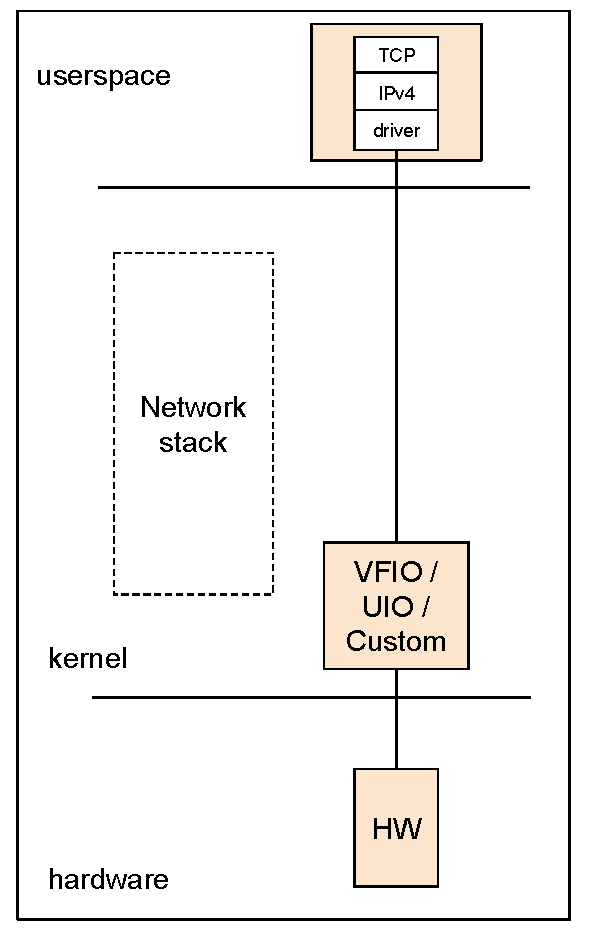
\includegraphics[width=\textwidth]{slides/networking-stack-overview/kernel_bypass.pdf}
		\column{0.7\textwidth}
	\begin{itemize}
		\item Contrary to \code{AF_PACKET}, Kernel Bypass techniques circumvent the networking stack
		\item Allows using an alternative implementation of the network stack, entirely running in userspace
			\begin{itemize}
				\item For use-case optimised scenarios
			\end{itemize}
		\item DPDK : Data Plate Development Kit
			\begin{itemize}
				\item Re-implement the drivers in userspace as well as a custom stack
			\end{itemize}
		\item Not supported by the linux kernel community
		\item Implies re-writing a full driver in userspace
		\item With \code{XDP} + \code{AF_XDP}, we now have a fully upstream solution
	\end{itemize}
	\end{columns}
\end{frame}

\begin{frame}{Netdev community}
	\begin{itemize}
		\item The networking stack is made of around 1M lines, 7000 distinct files
		\item 4 Maintainers share the top-level load :
			\begin{itemize}
				\item Jakub Kicinski, David S. Miller, Eric Dumazet and Paolo Abeni
			\end{itemize}
		\item Lots of maintainers for specific aspects of the networking stack
			\begin{itemize}
				\item Wireless, Bluetooth, TC, Ethernet framework, PHY framework, individual drivers...
			\end{itemize}
		\item Very active subsystem with lots of contributions and reviews.
	\end{itemize}
\end{frame}

\begin{frame}{Contributing}
	\begin{itemize}
		\item Development occurs on the \code{netdev@vger.kernel.org} mailing list, \href{https://lore.kernel.org/netdev/}{see archives}
		\item Follows the kernel development cycle, with a 2 weeks break during the merge window
		\item 2 git repositories are used as a development basis:
			\begin{itemize}
				\item \href{https://git.kernel.org/pub/scm/linux/kernel/git/netdev/net-next.git/}{net-next} : For \textbf{new features}, development stops during the Merge Window
					\begin{itemize}
						\item Check the \href{https://patchwork.hopto.org/net-next.html}{status page} before sending patches !
					\end{itemize}
				\item \href{https://git.kernel.org/pub/scm/linux/kernel/git/netdev/net.git/}{net} : For \textbf{fixes}, always open to patches.
			\end{itemize}
		\item Very fast-paced development, replies arrive quickly, for quick iterations
		\item Patch status can be tracked on \href{https://patchwork.kernel.org/project/netdevbpf/list/}{patchwork}
		\item Automated build-test and runtime tests are run with NIPA, results are published \href{https://netdev.bots.linux.dev/status.html}{here}
	\end{itemize}
\end{frame}

\begin{frame}{Conferences}
	\begin{itemize}
		\item The \href{https://lpc.events/}{\textbf{Linux Plumbers Conference}} hosts a Networking Track
			\begin{itemize}
				\item Main maintainers attend and host the track
				\item For \textbf{ongoing development}, to discuss current issues and future work
				\item Very technical topics
				\item Usually single-day track on a multi-day event
				\item LPC 2025 will be in Tôkyo, Japan, in December
			\end{itemize}
		\item The \href{https://netdevconf.info/}{\textbf{Netdev Conference}} is dedicated to kernel networking development
			\begin{itemize}
				\item Main maintainers also attend
				\item Hosted by a dedicated group of individuals (the Netdev Society)
				\item 4 or 5 days, mixing remte and on-site sessions
				\item Very technical topics as well, not many are embedded-oriented
				\item Netdev 2025 was in Zagreb, Croatia, in April.
			\end{itemize}
	\end{itemize}
\end{frame}

% Describe the approach of the linux net stack : 
% L2 -> L4 in kernel
% Rest in userspace
% Bypass
% Other stacks
% Maintainership
% Schematics of the net stack

